%%%%%%%%%%%%%%%%%%%%%%%%%%%%%%%%%%%%%%%%%%%%%%%%%%%%%%%%%%%%%%%%%%%%%
%
% CSCI 1430 Writeup Template
%
% This is a LaTeX document. LaTeX is a markup language for producing
% documents. Your task is to fill out this
% document, then to compile this into a PDF document.
%
% TO COMPILE:
% > pdflatex thisfile.tex
%
% For references to appear correctly instead of as '??', you must run
% pdflatex twice.
%
% If you do not have LaTeX and need a LaTeX distribution:
% - Departmental machines have one installed.
% - Personal laptops (all common OS): www.latex-project.org/get/
%
% If you need help with LaTeX, please come to office hours.
% Or, there is plenty of help online:
% https://en.wikibooks.org/wiki/LaTeX
%
% Good luck!
% James and the 1430 staff
%
%%%%%%%%%%%%%%%%%%%%%%%%%%%%%%%%%%%%%%%%%%%%%%%%%%%%%%%%%%%%%%%%%%%%%
%
% How to include two graphics on the same line:
%
% \includegraphics[\width=0.49\linewidth]{yourgraphic1.png}
% \includegraphics[\width=0.49\linewidth]{yourgraphic2.png}
%
% How to include equations:
%
% \begin{equation}
% y = mx+c
% \end{equation}
%
%%%%%%%%%%%%%%%%%%%%%%%%%%%%%%%%%%%%%%%%%%%%%%%%%%%%%%%%%%%%%%%%%%%%%%%%%%%%%%%%%%%%%%%%%%%%%%%%

\documentclass[11pt]{article}
\usepackage{vntex}
\usepackage[english]{babel}
\usepackage[utf8]{inputenc}
\usepackage[colorlinks = true,
            linkcolor = blue,
            urlcolor  = blue]{hyperref}
\usepackage[a4paper,margin=1.5in]{geometry}
\usepackage{stackengine,graphicx}
\usepackage{fancyhdr}
\setlength{\headheight}{15pt}
\usepackage{microtype}
\usepackage{times}
\usepackage{booktabs}
\usepackage{gensymb}
\usepackage{amsmath}
\usepackage{float}


% python code format: https://github.com/olivierverdier/python-latex-highlighting
\usepackage{pythonhighlight}

\frenchspacing
\setlength{\parindent}{0cm} % Default is 15pt.
\setlength{\parskip}{0.3cm plus1mm minus1mm}

\pagestyle{fancy}
\fancyhf{}
\lhead{Image Filtering and Hybrid Images}
\rhead{Xử lý ảnh số và thị giác máy tính}
\rfoot{\thepage}

\date{}

\title{\vspace{-1cm}Bài tập lớn 1: Image Filtering and Hybrid Images}


\begin{document}
\maketitle
\vspace{-2cm}
\thispagestyle{fancy}

\section*{Giới thiệu}
Bài tập lớn này tập trung vào việc hiện thực hàm tích chập (convolution) và sử dụng nó để sinh ra ảnh lai (hybrid image). Ảnh lai được xây dựng bằng cách pha trộn giữa tần số cao và tần số thấp của 2 ảnh khác nhau, chúng ta có thể tạo ra ảnh lại giữa hai ảnh ban đầu.

\section*{Chi tiết hiện thực}
\subsection*{Lọc ảnh}
Các bước hiện thực:
\begin{itemize}
    \item Xoay bộ lọc 180$^{\circ}$ trước khi thực hiện tích chập.
    \item Trên từng kênh màu:
        \begin{itemize}
            \item Thêm padding vào kênh màu để ảnh đầu ra có kích thước bằng với ảnh đầu vào.
            \item Áp dụng công thức tính dot product trên ma trận của ảnh và bộ lọc:
                \begin{equation*}
                    h[m,n] = \sum_{k,l} g[k,l]f[m+k,n+l]
                \end{equation*}
        \end{itemize}
\end{itemize}
Chi tiết hiện thực:
\inputpython{code/my_imfilter.py}{1}{45}

\subsection*{Ảnh lai}
Một ảnh lai (hybrid) là tổng của ảnh thứ nhất lọc bởi bộ lọc tần số thấp (low-pass filter) và ảnh thứ hai lọc bởi bộ lọc tần số cao (high-pass filter). Đối với hình ảnh đầu tiên, áp dụng bộ lọc để xóa sạch các thành phần có tần số cao hơn ngưỡng và bảo toàn phần tần số thấp. Mặt khác, áp dụng cùng một bộ lọc cho hình ảnh thứ hai, sau đó trừ hình ảnh được lọc ra khỏi hình ảnh gốc để loại bỏ phần tần số thấp. Kết hợp các hình ảnh và có được hình ảnh lai.

Chi tiết hiện thực:
\inputpython{code/hybrid_image.py}{1}{5}

\subsection*{Tích chập dựa trên biến đổi Fourier}
Hiện thực phép tích chập dựa theo công thức:
\begin{equation*}
    g*h=F^{-1}[F(g)F(h)]
\end{equation*}
Chi tiết hiện thực:
\inputpython{code/my_imfilter_fft.py}{1}{34}


\section*{Kết quả}
\subsection*{Lọc ảnh}
Ảnh 1:
\begin{figure}[h]
    \centering
    \includegraphics[width=5cm]{images/results_part1/cat/01_cat.jpg}
    \caption{Ảnh gốc}
\end{figure}

Ảnh sau khi lọc:
\begin{figure}[H]
    \centering
    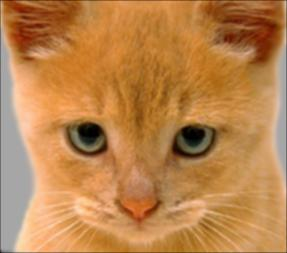
\includegraphics[width=5cm]{images/results_part1/cat/blur_image.jpg}
    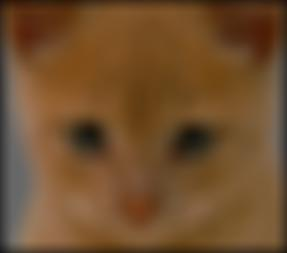
\includegraphics[width=5cm]{images/results_part1/cat/large_blur_image.jpg}
    \caption{\emph{Left:} Small blur. \emph{Right:} Large blur.}
\end{figure}

\begin{figure}[H]
    \centering
    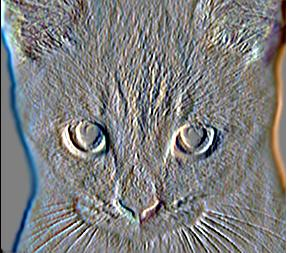
\includegraphics[width=5cm]{images/results_part1/cat/sobel_image.jpg}
    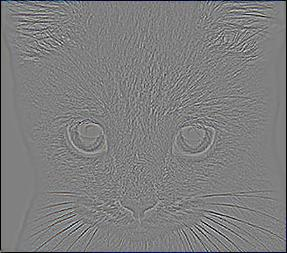
\includegraphics[width=5cm]{images/results_part1/cat/laplacian_image.jpg}
    \caption{\emph{Left:} Sobel image. \emph{Right:} Laplacian image.}
\end{figure}

\begin{figure}[H]
    \centering
    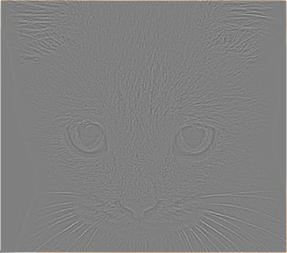
\includegraphics[width=5cm]{images/results_part1/cat/high_pass_image.jpg}
    \caption{High pass "filter"}
\end{figure}

Ảnh 2:
\begin{figure}[h]
    \centering
    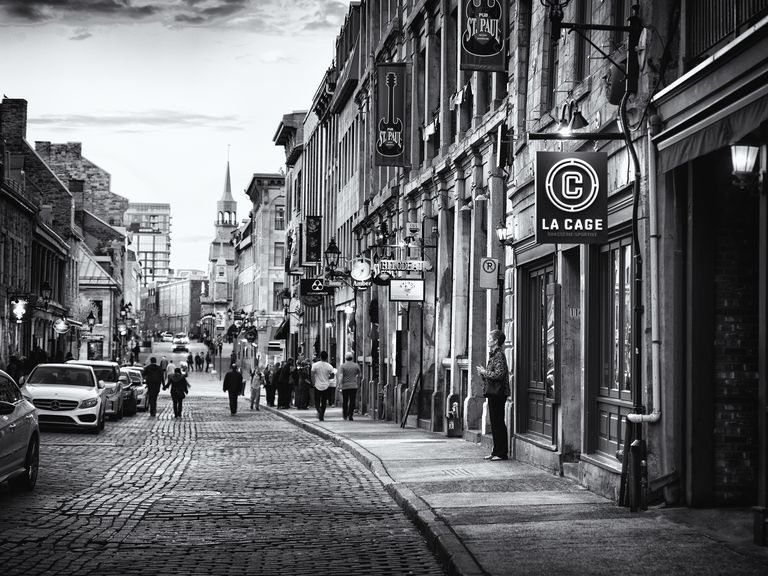
\includegraphics[width=5cm]{images/results_part1/image1/6_image1.jpg}
    \caption{Ảnh gốc}
\end{figure}

Ảnh sau khi lọc:
\begin{figure}[H]
    \centering
    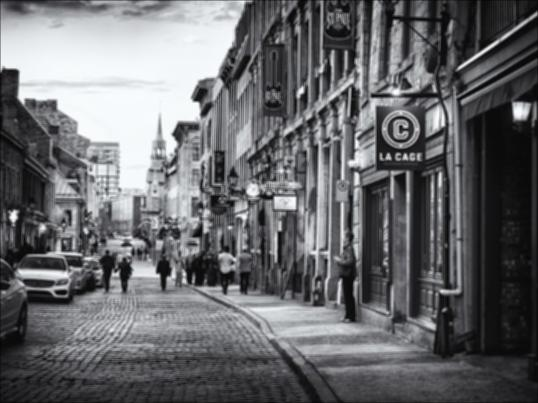
\includegraphics[width=5cm]{images/results_part1/image1/blur_image.jpg}
    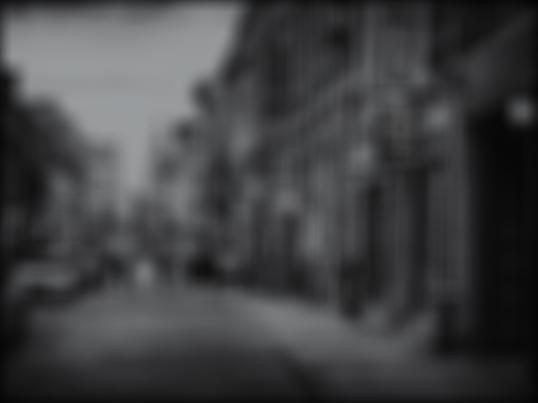
\includegraphics[width=5cm]{images/results_part1/image1/large_blur_image.jpg}
    \caption{\emph{Left:} Small blur. \emph{Right:} Large blur.}
\end{figure}

\begin{figure}[H]
    \centering
    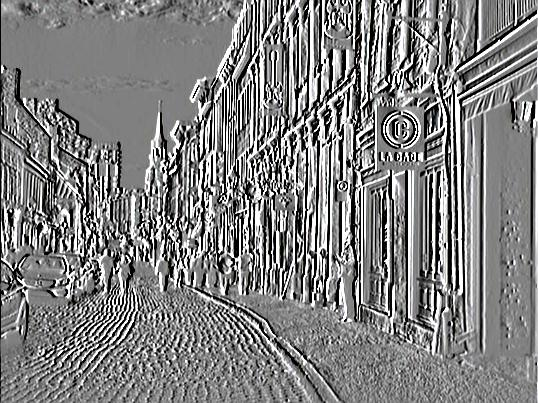
\includegraphics[width=5cm]{images/results_part1/image1/sobel_image.jpg}
    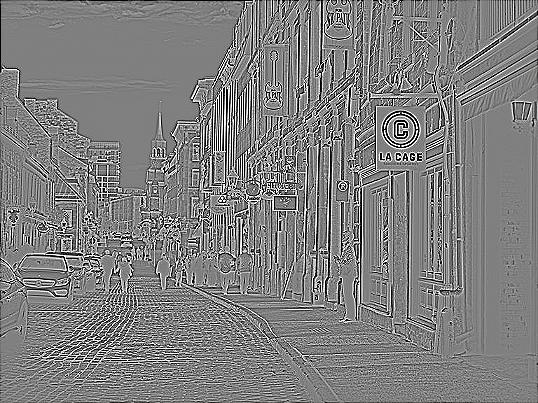
\includegraphics[width=5cm]{images/results_part1/image1/laplacian_image.jpg}
    \caption{\emph{Left:} Sobel image. \emph{Right:} Laplacian image.}
\end{figure}

\begin{figure}[H]
    \centering
    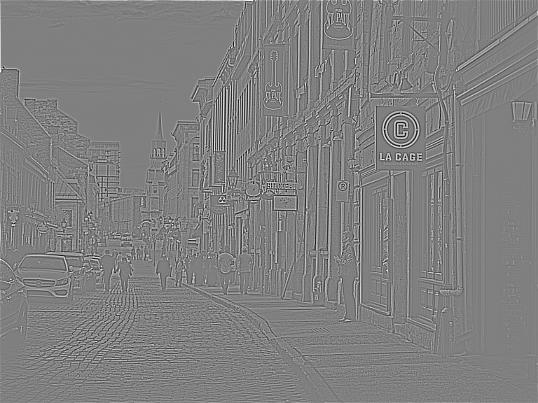
\includegraphics[width=5cm]{images/results_part1/image1/high_pass_image.jpg}
    \caption{High pass "filter"}
\end{figure}

\subsection*{Ảnh lai}
\text{Cặp ảnh 1:}
\begin{figure}[H]
    \centering
    \includegraphics[width=5cm]{images/results_part2/cat_dog/01_cat.jpg}
    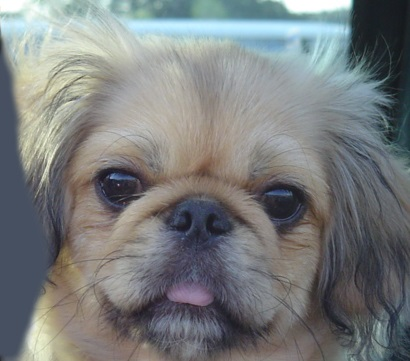
\includegraphics[width=5cm]{images/results_part2/cat_dog/01_dog.jpg}
    \caption{\emph{Left:} Ảnh gốc. \emph{Right:} Ảnh gốc.}
\end{figure}

\begin{figure}[H]
    \centering
    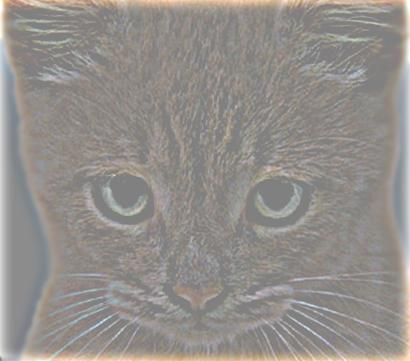
\includegraphics[width=5cm]{images/results_part2/cat_dog/high_frequencies.jpg}
    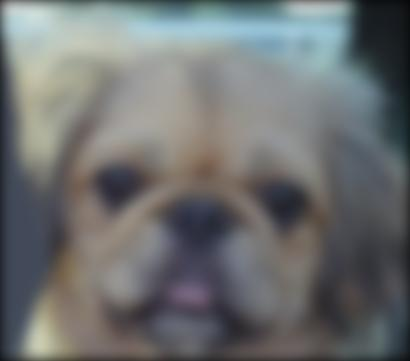
\includegraphics[width=5cm]{images/results_part2/cat_dog/low_frequencies.jpg}
    \caption{\emph{Left:} high-pass image. \emph{Right:} low-pass image.}
\end{figure}
\begin{figure}[H]
    \centering
    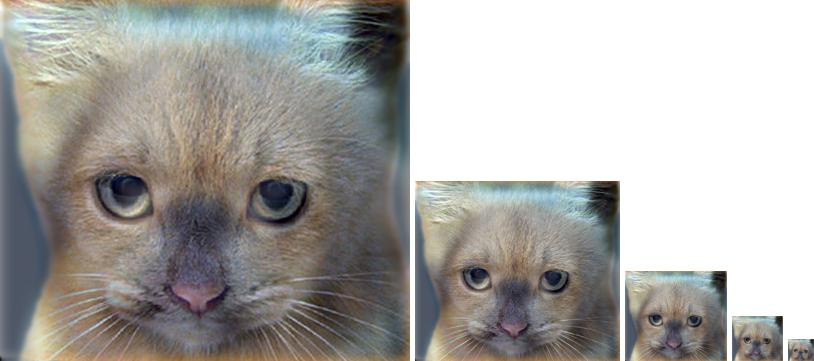
\includegraphics[width=10cm]{images/results_part2/cat_dog/hybrid_image_scales.jpg}
    \caption{Ảnh lai}
\end{figure}

\textbf{Cặp ảnh 2:}
\begin{figure}[H]
    \centering
    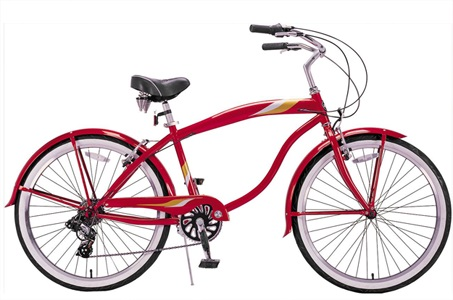
\includegraphics[width=5cm]{images/results_part2/motorcycle_bicycle/02_bicycle.jpg}
    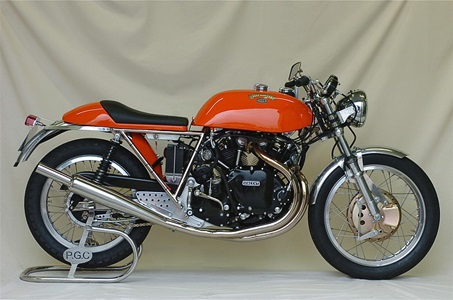
\includegraphics[width=5cm]{images/results_part2/motorcycle_bicycle/02_motorcycle.jpg}
    \caption{\emph{Left:} Ảnh gốc. \emph{Right:} Ảnh gốc.}
\end{figure}

\begin{figure}[H]
    \centering
    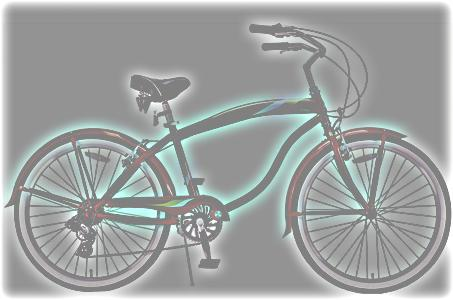
\includegraphics[width=5cm]{images/results_part2/motorcycle_bicycle/high_frequencies.jpg}
    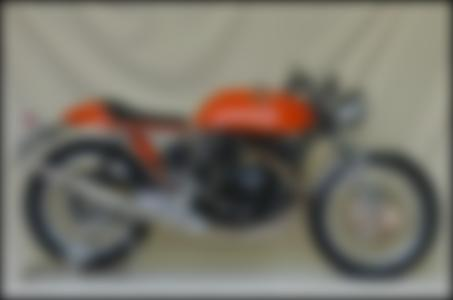
\includegraphics[width=5cm]{images/results_part2/motorcycle_bicycle/low_frequencies.jpg}
    \caption{\emph{Left:} high-pass image. \emph{Right:} low-pass image.}
\end{figure}
\begin{figure}[H]
    \centering
    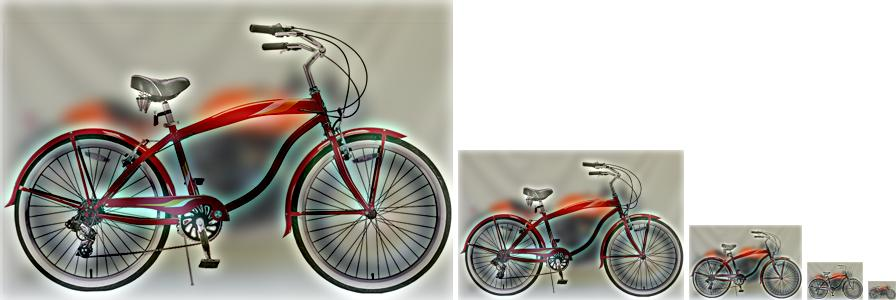
\includegraphics[width=10cm]{images/results_part2/motorcycle_bicycle/hybrid_image_scales.jpg}
    \caption{Ảnh lai}
\end{figure}

\textbf{Cặp ảnh 3:}
\begin{figure}[H]
    \centering
    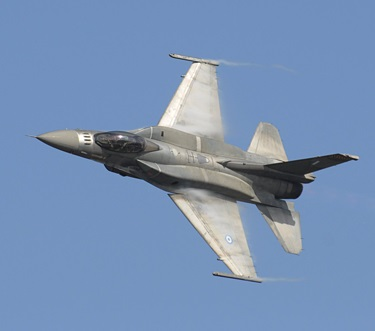
\includegraphics[width=5cm]{images/results_part2/bird_plane/03_plane.jpg}
    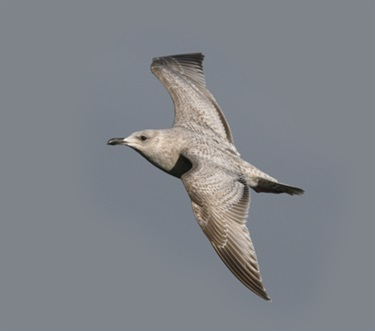
\includegraphics[width=5cm]{images/results_part2/bird_plane/03_bird.jpg}
    \caption{\emph{Left:} Ảnh gốc. \emph{Right:} Ảnh gốc.}
\end{figure}

\begin{figure}[H]
    \centering
    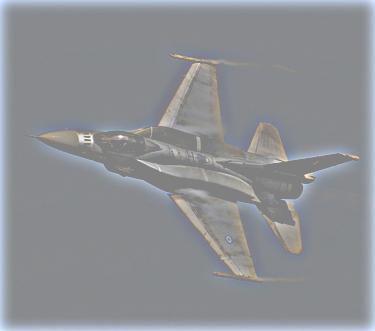
\includegraphics[width=5cm]{images/results_part2/bird_plane/high_frequencies.jpg}
    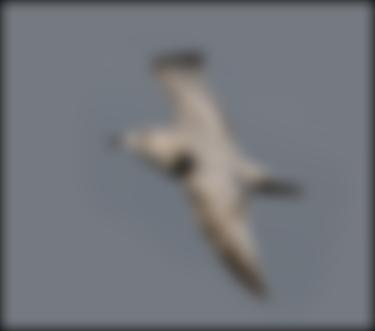
\includegraphics[width=5cm]{images/results_part2/bird_plane/low_frequencies.jpg}
    \caption{\emph{Left:} high-pass image. \emph{Right:} low-pass image.}
\end{figure}
\begin{figure}[H]
    \centering
    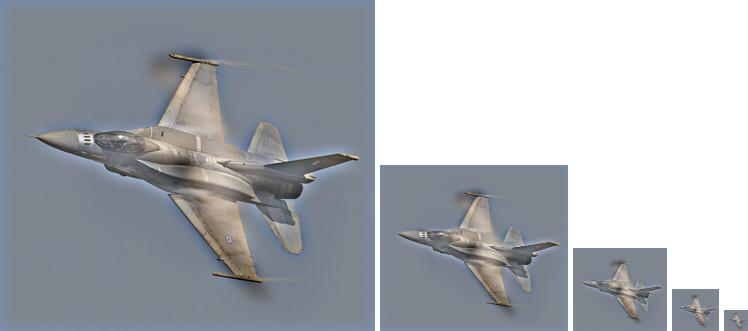
\includegraphics[width=10cm]{images/results_part2/bird_plane/hybrid_image_scales.jpg}
    \caption{Ảnh lai}
\end{figure}


\textbf{Cặp ảnh 4:}
\begin{figure}[H]
    \centering
    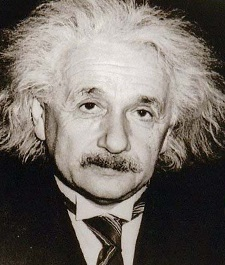
\includegraphics[width=5cm]{images/results_part2/marilyn_einstein/04_einstein.jpg}
    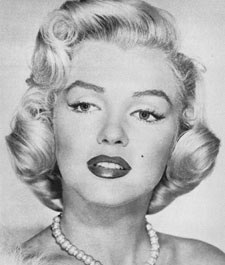
\includegraphics[width=5cm]{images/results_part2/marilyn_einstein/04_marilyn.jpg}
    \caption{\emph{Left:} Ảnh gốc. \emph{Right:} Ảnh gốc.}
\end{figure}

\begin{figure}[H]
    \centering
    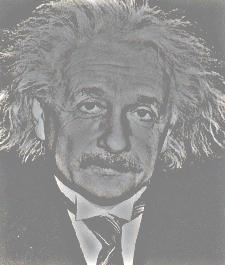
\includegraphics[width=5cm]{images/results_part2/marilyn_einstein/high_frequencies.jpg}
    
\includegraphics[width=5cm]{images/results_part2/marilyn_einstein/low_frequencies.jpg}
    \caption{\emph{Left:} high-pass image. \emph{Right:} low-pass image.}
\end{figure}
\begin{figure}[H]
    \centering
    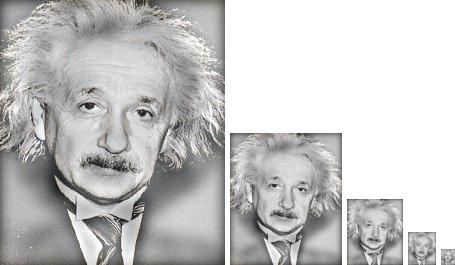
\includegraphics[width=10cm]{images/results_part2/marilyn_einstein/hybrid_image_scales.jpg}
    \caption{Ảnh lai}
\end{figure}

\textbf{Cặp ảnh 5:}
\begin{figure}[H]
    \centering
    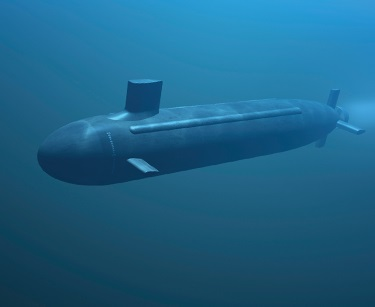
\includegraphics[width=5cm]{images/results_part2/fish_submarine/05_submarine.jpg}
    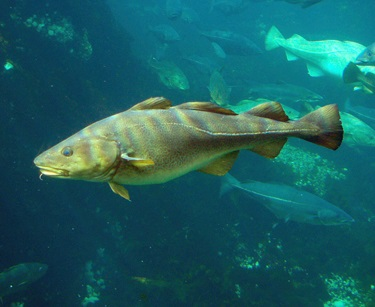
\includegraphics[width=5cm]{images/results_part2/fish_submarine/05_fish.jpg}
    \caption{\emph{Left:} Ảnh gốc. \emph{Right:} Ảnh gốc.}
\end{figure}

\begin{figure}[H]
    \centering
    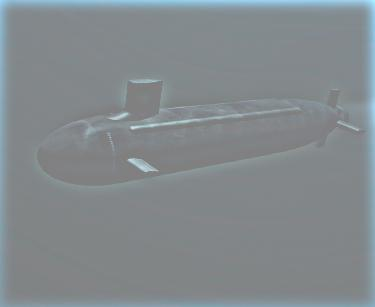
\includegraphics[width=5cm]{images/results_part2/fish_submarine/high_frequencies.jpg}
    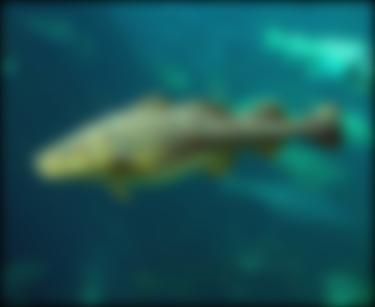
\includegraphics[width=5cm]{images/results_part2/fish_submarine/low_frequencies.jpg}
    \caption{\emph{Left:} high-pass image. \emph{Right:} low-pass image.}
\end{figure}
\begin{figure}[H]
    \centering
    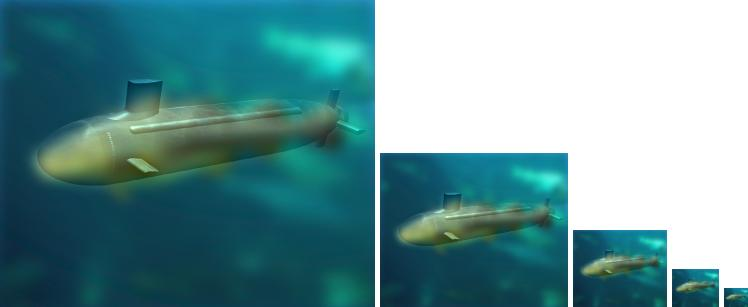
\includegraphics[width=10cm]{images/results_part2/fish_submarine/hybrid_image_scales.jpg}
    \caption{Ảnh lai}
\end{figure}

Kết quả so sánh giữa hai cách hiện thực convolution khác nhau trong bảng ~\ref{tab:table1} (đơn vị giây).

\begin{table}[h]
    \centering
    \begin{tabular}{|l|r|r|}
        \hline
                        & Basic convolution & Convolution using FFT\\
        \hline
        Lọc ảnh con mèo với gaussian filter & 3.4501  & 0.6921 \\
        \hline
        Lọc ảnh con mèo với nhiều bộ lọc trong part 1 & 8.4731  & 1.1128 \\
        \hline
        Tạo ảnh lai giữa ảnh chó và ảnh mèo & 11.1120  & 1.4636 \\
        \hline
    \end{tabular}
    \caption{Kết quả so sánh giữa hai cách hiện thực convolution khác nhau.}
    \label{tab:table1}
\end{table}

\end{document}
